\documentclass[border=6pt]{standalone}
\usepackage{tikz}
\usetikzlibrary{shapes.geometric, arrows.meta, positioning}
\begin{document}
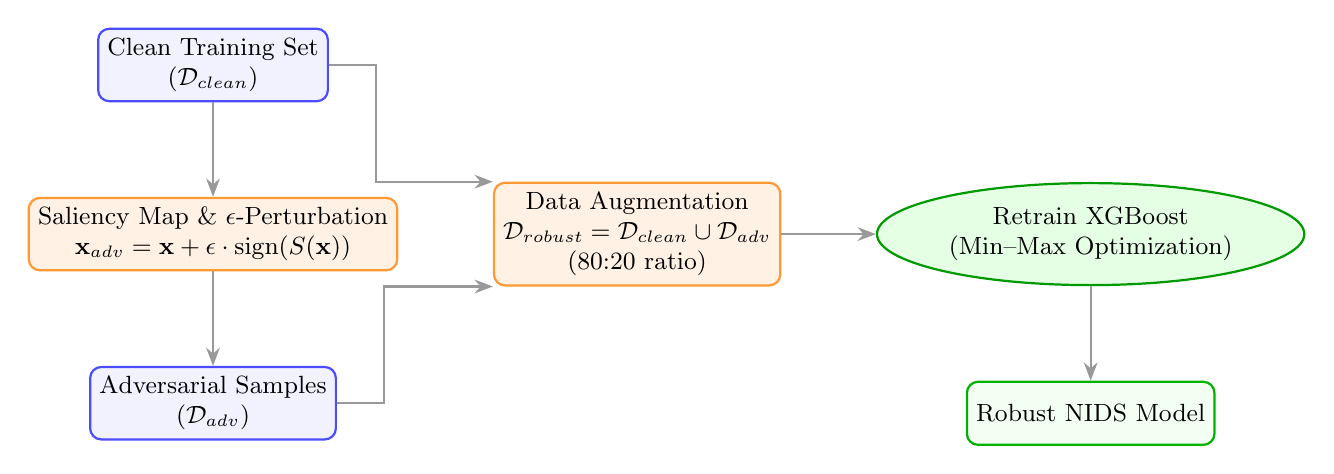
\begin{tikzpicture}[
    node distance=1.2cm and 1.5cm,
    block/.style={rectangle, draw=blue!70, fill=blue!5, thick, rounded corners, align=center, minimum height=0.8cm, font=\small},
    process/.style={rectangle, draw=orange!80, fill=orange!10, thick, rounded corners, align=center, minimum height=0.8cm, font=\small},
    model/.style={ellipse, draw=green!60!black, fill=green!10, thick, align=center, minimum height=0.8cm, font=\small},
    arrow/.style={-Stealth, thick, draw=gray!80}
]
    \node (clean) [block] {Clean Training Set\\($\mathcal{D}_{clean}$)};
    \node (saliency) [process, below=of clean] {Saliency Map \& $\epsilon$-Perturbation\\$\mathbf{x}_{adv} = \mathbf{x} + \epsilon \cdot \mathrm{sign}(S(\mathbf{x}))$};
    \node (adv_data) [block, below=of saliency] {Adversarial Samples\\($\mathcal{D}_{adv}$)};
    \node (combine) [process, right=1.2cm of saliency] {Data Augmentation\\$\mathcal{D}_{robust} = \mathcal{D}_{clean} \cup \mathcal{D}_{adv}$\\(80:20 ratio)};
    \node (retrain) [model, right=1.2cm of combine] {Retrain XGBoost\\(Min--Max Optimization)};
    \node (robust_model) [block, draw=green!70!black, fill=green!5, below=of retrain] {Robust NIDS Model};
    \draw [arrow] (clean) -- (saliency);
    \draw [arrow] (saliency) -- (adv_data);
    \draw [arrow] (clean.east) -- ++(0.6,0) |- (combine.north west);
    \draw [arrow] (adv_data.east) -- ++(0.6,0) |- (combine.south west);
    \draw [arrow] (combine) -- (retrain);
    \draw [arrow] (retrain) -- (robust_model);
\end{tikzpicture}
\end{document}
